\documentclass[11pt]{article}

% ---------------------------------------------------------------- packages
\usepackage[a4paper,margin=1in]{geometry}
\usepackage[T1]{fontenc}
\usepackage{mathptmx}
\usepackage{amsmath,amssymb}
\usepackage{microtype}
\usepackage{graphicx}
\usepackage{booktabs,multirow,makecell}
\usepackage[font=small,labelfont=bf]{caption}
\usepackage{subcaption}
\usepackage{xcolor}
\usepackage{enumitem}
\usepackage{float}
\usepackage{tikz}
\usetikzlibrary{arrows.meta,positioning,fit}
\usepackage[numbers,sort&compress]{natbib}
\usepackage[colorlinks=true,linkcolor=blue!50!black,citecolor=blue!50!black,urlcolor=blue!50!black]{hyperref}

\setlist{itemsep=2pt,topsep=4pt}
\graphicspath{{../figures/}}
\newcommand{\figref}[1]{Fig.~\ref{#1}}
\newcommand{\tabref}[1]{Table~\ref{#1}}
\newcommand{\secref}[1]{Section~\ref{#1}}

\title{\textbf{Does Restoration Help Detection?}\\[2pt]
\large A Controlled Study of Denoising, Deblocking and Low-Light Enhancement\\ for Object Detection}
\author{Shourja Banerjee\\[2pt]
\small B.Tech.\ Computer Science and Engineering\\
\small \url{https://github.com/onigiri4711/degrade-restore-detect}}
\date{November 2026}

\begin{document}
\maketitle

% ================================================================= abstract
\begin{abstract}
\noindent
Image restoration methods are usually judged by pixel-fidelity metrics such as PSNR, but restored images are increasingly consumed by machines rather than people. We ask whether restoration actually helps a pretrained object detector, and whether PSNR predicts which restorer helps most. We build seven seeded degradation models and evaluate tuned classical filters, BM3D, contrast enhancement, matched inverses and a blind DnCNN that we train from scratch, first on 96 held-out BSD500 images and then with YOLOv8n on 300 COCO val2017 images under Gaussian noise, JPEG compression and low light. A strong denoiser recovers about three-quarters of the mAP lost to Gaussian noise (DnCNN 70--83\%, BM3D 70--76\%), against 27--60\% for tuned simple filters. DnCNN leads BM3D by 0.6--1.8\,dB in PSNR, but their detection results are statistically indistinguishable. JPEG restoration helps only at strong compression. In low light, PSNR is misleading: contrast enhancement and gamma brightening raise PSNR but \emph{lower} mAP by amplifying noise, while brightening followed by denoising recovers 35--67\% of the lost mAP and is best at every level. Paired bootstrap intervals show that most differences are statistically clear, yet a restorer's PSNR gain on an image barely predicts its detection gain on that image (Spearman $-0.14$ to $+0.21$). An analysis of the trained network shows that it learned colour-opponent filters and a noise-adaptive receptive field, and that it fails along strong edges on damage it was never trained on. We conclude that restoration for machine perception should be evaluated with the downstream task metric.
\end{abstract}

% ================================================================= 1 intro
\section{Introduction}
\label{sec:intro}

Images reach vision systems damaged. Small sensors add noise, storage and transmission add compression artifacts, and poor lighting leaves images dark and noisy. A large literature restores such images, from classical filters~\citep{tomasi1998bilateral,buades2005nlmeans,dabov2007bm3d} to deep networks~\citep{zhang2017dncnn,zhang2018ffdnet,guo2019cbdnet}, and almost all of it is evaluated with PSNR or SSIM~\citep{wang2004ssim} against a clean reference. These metrics reward closeness to the original pixels. A downstream model such as an object detector, however, depends on edges, shapes and textures, and it is not obvious that the restoration a pixel metric prefers is the one that serves the detector best. A denoiser that wins on PSNR by smoothing everything could erase exactly the structure a detector relies on.

This paper asks a simple question in a controlled setting: \textbf{as images become noisier, more compressed or darker, how much does a pretrained detector's accuracy fall, how much of the loss does each restoration method recover, and does the restorer with the best PSNR also recover the most detection accuracy?}

We answer it with a three-stage pipeline (\figref{fig:pipeline}): \emph{degrade} clean images with seeded, physically motivated models; \emph{restore} them with classical and learned methods; and \emph{detect} objects with a pretrained YOLOv8n~\citep{jocher2023yolov8}, scored with COCO mAP~\citep{lin2014coco}. Every method sees the identical damaged image, so all comparisons are paired. We wrote down five hypotheses before running the detection experiments, and we test differences with paired bootstrap confidence intervals~\citep{efron1979bootstrap}.

\paragraph{Contributions.}
\begin{itemize}
  \item A controlled, paired evaluation of restoration for detection across three degradations and twelve severity levels, with ten restorers and pipelines and bootstrap confidence intervals for every comparison (\secref{sec:det}).
  \item Evidence that a strong denoiser (DnCNN or BM3D) recovers about three-quarters of the mAP lost to Gaussian noise, and that DnCNN's sizeable PSNR lead over BM3D does \emph{not} translate into a detection advantage (\secref{sec:bm3d}).
  \item A low-light result in which PSNR ranks methods in the wrong order: brightening raises PSNR and lowers mAP, while brightening \emph{followed by} denoising is best, and the order of the two steps matters (\secref{sec:lowlight}).
  \item An analysis of what the trained DnCNN learned (filters, effective receptive field, frequency response, residuals) that explains both its successes and its failures (\secref{sec:interp}).
  \item From-scratch NumPy implementations of a JPEG codec and a convolution layer with backpropagation, verified against libjpeg and numerical gradients (Appendix~\ref{app:scratch}).
\end{itemize}

\begin{figure}[t]
\centering
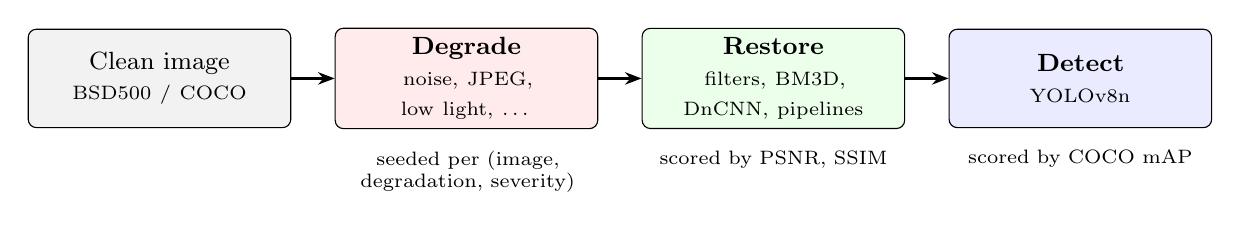
\begin{tikzpicture}[
  box/.style={draw, rounded corners=3pt, align=center, minimum height=1.25cm, text width=3.1cm, font=\small, fill=#1},
  arr/.style={-{Stealth[length=6pt]}, thick},
  lab/.style={font=\scriptsize, align=center, text width=3.2cm}]
\node[box=gray!10] (clean) {Clean image\\{\scriptsize BSD500 / COCO}};
\node[box=red!8, right=0.55cm of clean] (deg) {\textbf{Degrade}\\{\scriptsize noise, JPEG, low light, \dots}};
\node[box=green!8, right=0.55cm of deg] (res) {\textbf{Restore}\\{\scriptsize filters, BM3D, DnCNN, pipelines}};
\node[box=blue!8, right=0.55cm of res] (det) {\textbf{Detect}\\{\scriptsize YOLOv8n}};
\draw[arr] (clean) -- (deg); \draw[arr] (deg) -- (res); \draw[arr] (res) -- (det);
\node[lab, below=0.15cm of deg] {seeded per (image,\\degradation, severity)};
\node[lab, below=0.15cm of res] {scored by PSNR, SSIM};
\node[lab, below=0.15cm of det] {scored by COCO mAP};
\end{tikzpicture}
\caption{The degrade $\rightarrow$ restore $\rightarrow$ detect pipeline. Every restorer receives the identical damaged image, so differences between restorers are paired. Each restored image receives two scores: pixel fidelity (PSNR) and detection accuracy (mAP).}
\label{fig:pipeline}
\end{figure}

% ================================================================= 2 related
\section{Related Work}
\label{sec:related}

\paragraph{Classical restoration.}
Linear smoothing and the median filter are the textbook denoisers~\citep{gonzalez2018dip}. The bilateral filter~\citep{tomasi1998bilateral} averages only neighbours of similar intensity, preserving edges, and non-local means~\citep{buades2005nlmeans} averages patches that look alike anywhere in a search window. BM3D~\citep{dabov2007bm3d} groups similar patches into 3-D stacks and shrinks them jointly in a transform domain, and it remained the reference non-learned denoiser for a decade. Noise level can be estimated blindly from the finest wavelet band with the median absolute deviation~\citep{donoho1994wavelet}. Blur is inverted by Wiener deconvolution~\citep{gonzalez2018dip}, colour casts by gray-world white balance~\citep{buchsbaum1980grayworld}, and low contrast by histogram equalisation and its contrast-limited adaptive form, CLAHE~\citep{pizer1987ahe,zuiderveld1994clahe}.

\paragraph{Learned restoration.}
DnCNN~\citep{zhang2017dncnn} showed that a deep CNN with batch normalisation~\citep{ioffe2015bn} trained to predict the noise residual outperforms BM3D, and that one network can denoise blindly across noise levels. FFDNet~\citep{zhang2018ffdnet} conditions on a noise map, and CBDNet~\citep{guo2019cbdnet} models realistic camera noise. Learned low-light enhancement includes Retinex-based decomposition~\citep{wei2018retinexnet} and zero-reference curve estimation~\citep{guo2020zerodce}. We train a blind DnCNN as our learned restorer because it is simple, well understood and reproducible on a single GPU.

\paragraph{Quality metrics.}
PSNR measures mean squared error on a log scale; SSIM~\citep{wang2004ssim} compares local luminance, contrast and structure; LPIPS~\citep{zhang2018lpips} compares deep features and tracks human judgements better. None of them is designed to predict the performance of a downstream model, which is the gap this study examines.

\paragraph{Robustness of recognition to image degradation.}
Deep classifiers degrade sharply under noise and blur~\citep{dodge2016quality}, and standardised corruption benchmarks exist for classification~\citep{hendrycks2019benchmarking} and detection~\citep{michaelis2019winter}. The ExDark dataset~\citep{loh2019exdark} provides object labels in real low light. These works measure how much accuracy is lost; we measure how much restoration wins back, and whether pixel metrics predict it.

\paragraph{Restoration for high-level vision.}
\citet{liu2018denoising} train a denoiser jointly with a high-level vision loss and show that pixel-optimal denoising is not task-optimal. \citet{diamond2021dirty} optimise the image-processing pipeline end to end for classification. Our study is complementary: rather than proposing a task-driven method, we run a controlled, paired comparison of standard restorers, quantify its uncertainty, and explain the outcome with an analysis of the restorer itself, in the spirit of filter visualisation~\citep{zeiler2014visualizing} and effective-receptive-field analysis~\citep{luo2016erf}.

% ================================================================= 3 method
\section{Method}
\label{sec:method}

\subsection{Degradation models}
\label{sec:degradations}
Images are float32 RGB in $[0,1]$. Each degradation is a function of the clean image $x$, a severity $s$ and a random generator, and the result is clipped to $[0,1]$ once, as a sensor saturates. The generator is seeded from (image index, degradation index, severity index), so every restorer receives the identical damaged image. \tabref{tab:degradations} lists the models. The low-light model is our own: it darkens with a gamma curve and then adds signal-dependent shot noise and read noise, and it reduces to the identity at $\ell=0$. A statistical test checks each model before any experiment (for example, Gaussian residuals must have standard deviation $\sigma/255$ within 3\%, and Poisson variance must equal $x/p$ within 5\%); all nine checks pass.

\begin{table}[t]
\centering\small
\caption{Degradation models. Severities run from mild to severe; the detection study uses Gaussian noise, JPEG and low light.}
\label{tab:degradations}
\begin{tabular}{@{}lll@{}}
\toprule
Degradation & Model & Severities \\
\midrule
Gaussian noise & $y = x + n,\; n \sim \mathcal{N}(0, (\sigma/255)^2)$ i.i.d. & $\sigma = 5, 15, 25, 35, 50$ \\
Poisson noise & $y = \mathrm{Poisson}(p\,x)/p$ & $p = 100, 50, 20, 10, 5$ \\
Salt and pepper & fraction $a$ of pixels set to 0 or 1 & $a = 0.01$--$0.2$ \\
Blur & Gaussian kernel of std $\sigma$ px & $\sigma = 0.5$--$3$ \\
JPEG & encode and decode at quality $q$ & $q = 90, 70, 50, 30, 10$ \\
Colour cast & channel gains $(1+s, 1, 1-s)$ & $s = 0.1$--$0.5$ \\
Low light & $x_d = (1-0.8\ell)\,x^{1+2\ell}$, then shot noise (peak $200(1-\ell)+5$) & $\ell = 0.2$--$0.9$ \\
 & and read noise (std $0.01 + 0.04\ell$) & \\
\bottomrule
\end{tabular}
\end{table}

\subsection{Restorers}
\label{sec:restorers}

\paragraph{Tuned classical filters.} Gaussian, median, bilateral and non-local-means filters are tuned by grid search on four BSD500 validation images for every (degradation, severity), and the tuned settings are applied to the remaining 96. Because they are tuned for each severity, these filters effectively know the noise level (an \emph{oracle} advantage), which makes them an upper bound for their class. We also report a \emph{blind} NL-means whose strength is set from a wavelet-based noise estimate~\citep{donoho1994wavelet}.

\paragraph{BM3D.} We use the reference implementation~\citep{dabov2007bm3d} for colour images, given the true $\sigma$ (also an oracle).

\paragraph{Contrast enhancement and matched inverses.} Global histogram equalisation (HE) and CLAHE~\citep{zuiderveld1994clahe} are applied to the L channel of Lab, which leaves colour unchanged. Gray-world white balance~\citep{buchsbaum1980grayworld} corrects colour casts, and Wiener deconvolution $\hat{X} = \frac{H^*}{|H|^2 + K}\,Y$ inverts blur (Appendix~\ref{app:classical}).

\paragraph{DnCNN.} We train a blind colour DnCNN~\citep{zhang2017dncnn} that predicts the noise residual $\hat{v}=f(y)$ and outputs $y-\hat{v}$. It has 17 convolutional layers of $3\times3$ kernels with 64 channels and batch normalisation, 558{,}403 parameters and a theoretical receptive field of $35\times35$ pixels. Training uses the 400 BSDS500~\citep{arbelaez2011bsds500} train and test images at four scales, cut into about 381{,}000 patches of $40\times40$ pixels. Each patch receives a random flip or rotation and fresh Gaussian noise with $\sigma \sim \mathcal{U}[0,55]$, clipped to $[0,1]$ to match the evaluation pipeline. We minimise the MSE between predicted and true noise with Adam~\citep{kingma2015adam} (learning rate $10^{-3}$, divided by 10 at 60\% and 85\% of 50 epochs, batch size 128) on one T4 GPU, taking 3.8 hours. The 100 BSD500 validation images, which contain the standard CBSD68 benchmark, are held out; a check by file name and pixel hash finds no overlap with training. DnCNN never sees JPEG or low-light images, so those conditions test generalisation.

\paragraph{Low-light pipelines.} To test \emph{why} contrast enhancement fails in low light, we add a blind gamma curve that raises every channel to the power $g = \log 0.45 / \log \bar{Y}$, where $\bar{Y}$ is the image's mean luma, and we combine it with DnCNN and CLAHE in both orders: gamma$\to$DnCNN, DnCNN$\to$gamma, DnCNN$\to$CLAHE and CLAHE$\to$DnCNN.

\subsection{Detection protocol}
\label{sec:protocol}
A pretrained YOLOv8n~\citep{redmon2016yolo,jocher2023yolov8} is evaluated with the official COCO mAP@[.5:.95] on a fixed random subset of 300 COCO val2017 images containing 2{,}035 objects (808 small, 697 medium, 530 large). Detections are kept down to confidence $10^{-3}$ so that mAP integrates the full precision--recall curve. Its 80 class indices are mapped to COCO's non-contiguous category ids. Clean mAP on the subset is 0.387, in line with the published 0.373 on the full validation set. Each image is degraded with Gaussian noise ($\sigma = 15, 25, 35, 50$), JPEG ($q = 70, 50, 30, 10$) or low light ($\ell = 0.4, 0.6, 0.8, 0.9$), using the same functions and seeds as the restoration experiments. To compare conditions we report the \emph{share of lost mAP recovered},
\begin{equation}
R = \frac{\mathrm{mAP}_{\text{restored}} - \mathrm{mAP}_{\text{damaged}}}{\mathrm{mAP}_{\text{clean}} - \mathrm{mAP}_{\text{damaged}}},
\end{equation}
where $R=100\%$ means detection returns to the clean level and $R<0$ means the restoration made it worse.

\paragraph{Hypotheses.} Before running the detection experiments we wrote down five hypotheses based on the restoration results:
\textbf{H1}: mAP falls steadily with severity.
\textbf{H2}: on Gaussian noise both restorers recover much of the lost mAP, DnCNN more.
\textbf{H3}: on JPEG little is recovered, and DnCNN may hurt.
\textbf{H4}: in low light, CLAHE helps more than any denoiser.
\textbf{H5}: in some condition, the restorer with the best PSNR is not the one with the best mAP.

\subsection{Statistical analysis}
\label{sec:stats}
COCO mAP pools detections across images, so it cannot be cheaply recomputed on a resample. We therefore bootstrap the \emph{image-averaged AP}, the mean of each image's own AP, which ranks all 65 runs the same way as COCO mAP (Spearman 0.997). We draw 10{,}000 resamples of the 300 images with replacement and use the same resamples for every run, so the difference between two restorers is a \emph{paired} bootstrap. A difference is called \emph{clear} when its 95\% percentile interval excludes zero.

\subsection{Interpretability probes}
\label{sec:probes}
We inspect the trained DnCNN in five ways: (i) the cosine similarity of each first-layer filter to textbook kernels (Gaussian, Laplacian, Sobel, identity) and the share of its energy in differences between colour channels; (ii) the effective receptive field~\citep{luo2016erf}, measured as the gradient of one output pixel with respect to every input pixel; (iii) an average transfer function, the ratio of output to input power spectra; (iv) the predicted residual on inputs outside the training distribution; and (v) a gallery of images where DnCNN has the higher PSNR but the lower detection AP.

% ================================================================= 4 results
\section{Results}
\label{sec:results}

\subsection{Restoration quality}
\label{sec:psnr}
Classical filters split cleanly into two groups (Appendix~\ref{app:classical}). On the three noise degradations they gain 7--11\,dB at mid severity, with the winner matching each filter's assumption (median for impulse noise, bilateral for Gaussian and Poisson noise). On blur, colour cast, low light and JPEG no filter gains more than 0.6\,dB, because these are not random errors; their matched inverses (Wiener, gray-world) gain up to 9.5 and 7.7\,dB.

\begin{table}[t]
\centering\small
\caption{PSNR (dB) on the 96 held-out BSD500 images under Gaussian noise. ``Oracle'' methods are given the true $\sigma$; DnCNN is blind.}
\label{tab:psnr}
\begin{tabular}{@{}cccccc@{}}
\toprule
$\sigma$ & Noisy & Blind NL-means & Tuned filter (oracle) & BM3D (oracle) & DnCNN (blind) \\
\midrule
15 & 24.82 & 28.33 & 30.90 & 33.20 & \textbf{33.76} \\
25 & 20.53 & 25.59 & 27.56 & 30.18 & \textbf{31.05} \\
50 & 15.00 & 22.63 & 23.20 & 25.92 & \textbf{27.69} \\
\bottomrule
\end{tabular}
\end{table}

On Gaussian noise (\tabref{tab:psnr}), DnCNN beats the best tuned filter by 2.9--4.5\,dB and BM3D by 0.6--1.8\,dB, and the gap grows with the noise level, the same pattern reported in the DnCNN paper. Our DnCNN is within 0.1--0.2\,dB of the published blind colour model on CBSD68 (33.89, 31.23 and 27.92\,dB)~\citep{zhang2017dncnn}. It improves every test image at every level, and it degrades gracefully beyond its training range (26.16 and 24.56\,dB at $\sigma = 65$ and 75).

\subsection{Detection under degradation}
\label{sec:det}

\begin{table}[t]
\centering\small
\caption{YOLOv8n mAP@[.5:.95] on 300 COCO val2017 images (clean: 0.387). Best per row in bold. ``Tuned'' is the classical filter tuned for that exact condition; gamma$\to$DnCNN brightens first, then denoises.}
\label{tab:map}
\begin{tabular}{@{}llcccccc@{}}
\toprule
Degradation & Severity & None & Tuned & BM3D & DnCNN & CLAHE & gamma$\to$DnCNN \\
\midrule
\multirow{4}{*}{Gaussian} & $\sigma=15$ & 0.319 & 0.359 & 0.371 & \textbf{0.375} & -- & -- \\
 & $\sigma=25$ & 0.241 & 0.305 & 0.343 & \textbf{0.354} & -- & -- \\
 & $\sigma=35$ & 0.181 & 0.264 & \textbf{0.327} & 0.326 & -- & -- \\
 & $\sigma=50$ & 0.088 & 0.169 & 0.297 & \textbf{0.304} & -- & -- \\
\midrule
\multirow{4}{*}{JPEG} & $q=70$ & 0.376 & \textbf{0.378} & -- & \textbf{0.378} & -- & -- \\
 & $q=50$ & 0.349 & \textbf{0.366} & -- & 0.348 & -- & -- \\
 & $q=30$ & 0.309 & \textbf{0.346} & -- & 0.305 & -- & -- \\
 & $q=10$ & 0.125 & \textbf{0.231} & -- & 0.121 & -- & -- \\
\midrule
\multirow{4}{*}{Low light} & $\ell=0.4$ & 0.274 & 0.286 & -- & 0.325 & 0.250 & \textbf{0.349} \\
 & $\ell=0.6$ & 0.207 & 0.226 & -- & 0.283 & 0.174 & \textbf{0.305} \\
 & $\ell=0.8$ & 0.121 & 0.134 & -- & 0.213 & 0.095 & \textbf{0.242} \\
 & $\ell=0.9$ & 0.056 & 0.088 & -- & 0.159 & 0.044 & \textbf{0.172} \\
\bottomrule
\end{tabular}
\end{table}

\begin{figure}[t]
\centering
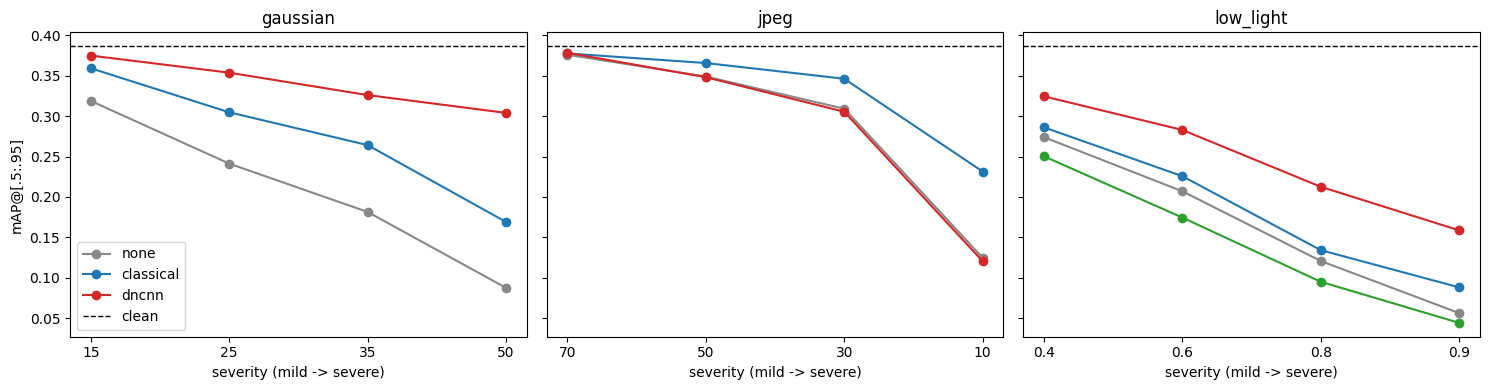
\includegraphics[width=\linewidth]{fig17_map_vs_severity.png}
\caption{mAP against severity for each restorer from the main sweep. The dashed line is clean mAP. On Gaussian noise DnCNN stays close to clean mAP up to $\sigma=50$; on JPEG it tracks the unrestored curve; in low light CLAHE falls below no restoration.}
\label{fig:map}
\end{figure}

\tabref{tab:map} and \figref{fig:map} summarise the detection results. Every degradation lowers mAP at every step (H1 confirmed), to 0.088 at $\sigma = 50$, 0.125 at $q=10$ and 0.056 at $\ell=0.9$.

\textbf{Gaussian noise.} DnCNN recovers 70--83\% of the lost mAP at every $\sigma$, while the tuned filter's share falls from 60\% to 27\% as noise grows; at $\sigma=50$ DnCNN keeps 0.304 against the filter's 0.169 (H2 confirmed against simple filters).

\textbf{JPEG.} DnCNN, which never saw block artifacts, never helps: its recovered share ranges from $-5\%$ to $+23\%$, the larger value at $q=70$ where almost nothing was lost. The bilateral filter recovers 41--48\% of the lost mAP at $q=30$ and $10$ while raising PSNR by only 0.4--0.5\,dB: smoothing the $8\times8$ block edges removes false edges the detector would otherwise respond to. At $q=50$ and 70 its gain is not statistically clear (H3 confirmed, except at strong compression).

\textbf{Low light.} CLAHE makes detection worse than doing nothing at every level ($-4\%$ to $-21\%$), although it has the highest PSNR of the single methods. DnCNN, outside its training distribution, is the best single method (31--45\%), and brightening followed by DnCNN is best overall (H4 rejected; \secref{sec:lowlight}).

\subsection{How sure are we? Paired bootstrap intervals}
\label{sec:ci}

\begin{figure}[t]
\centering
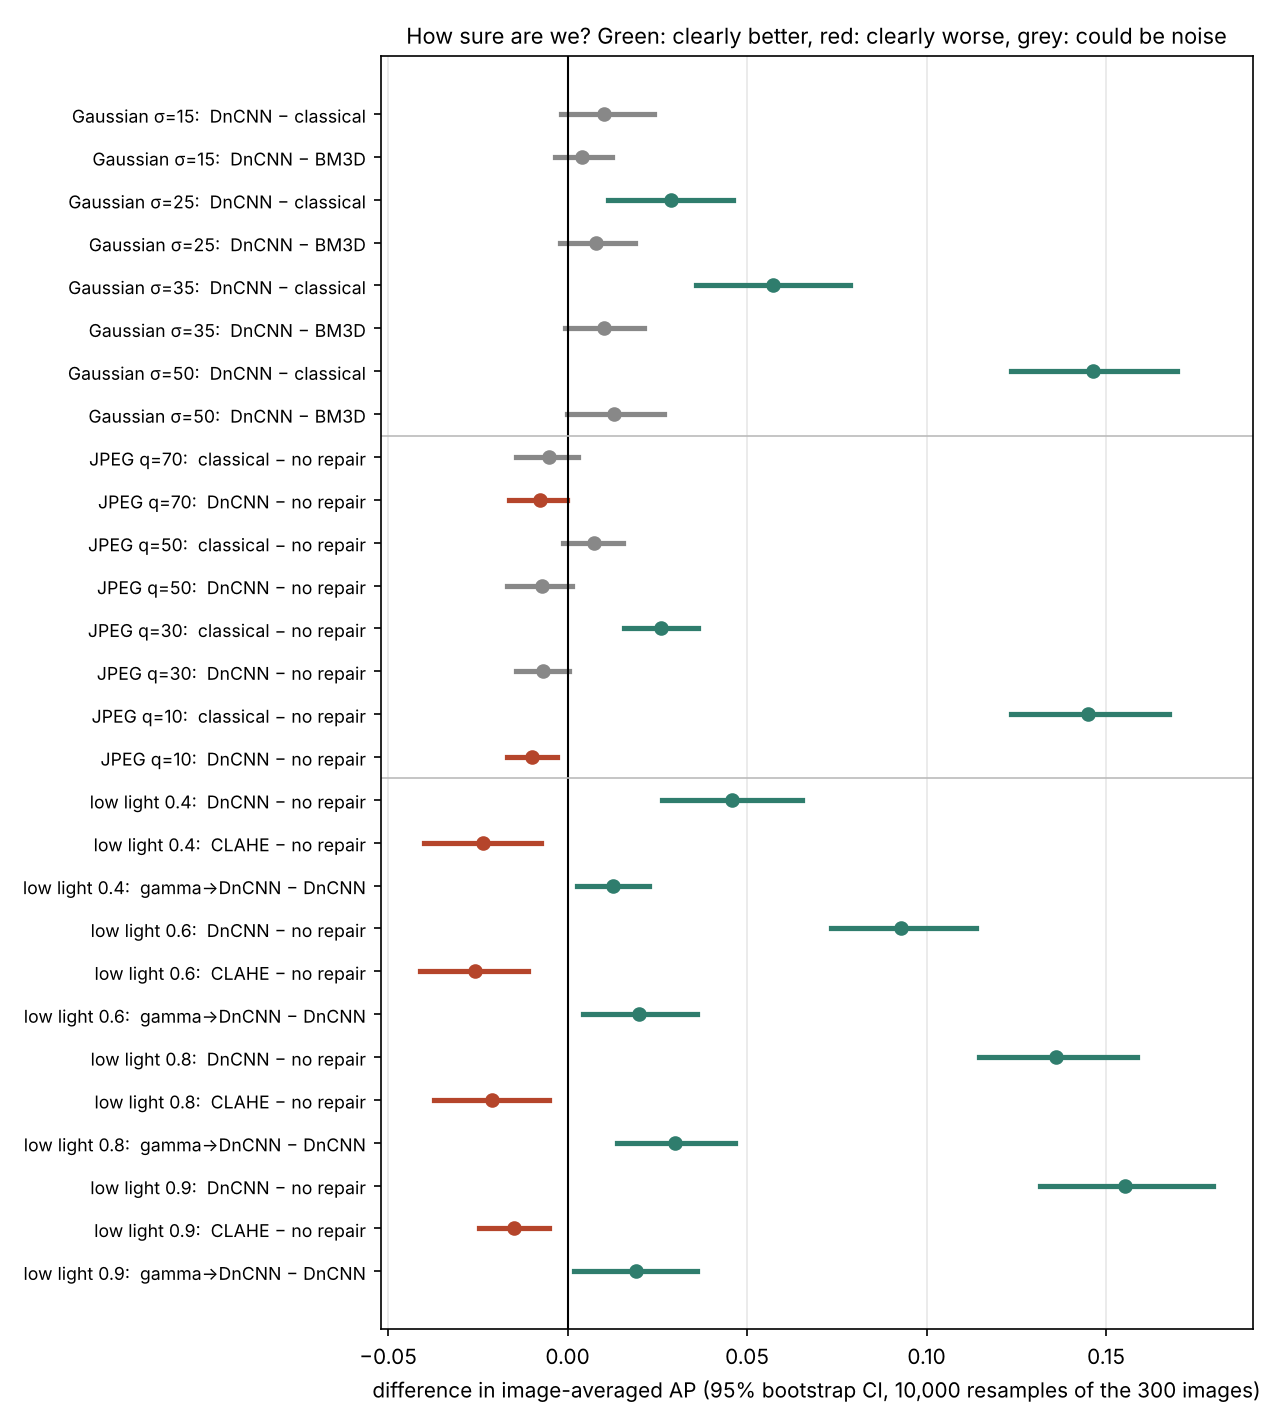
\includegraphics[width=0.78\linewidth]{fig24_bootstrap_ci.png}
\caption{Key paired differences in image-averaged AP, with 95\% bootstrap intervals from 10{,}000 resamples of the 300 images. Green: clearly better; red: clearly worse; grey: could be noise.}
\label{fig:ci}
\end{figure}

\figref{fig:ci} shows the key comparisons. DnCNN's lead over the tuned filter is clear from $\sigma = 25$ upward ($+0.029$, $+0.057$, $+0.146$) but not at $\sigma=15$ ($+0.010$, interval $-0.002$ to $+0.024$). DnCNN's small JPEG losses ($-0.007$ to $-0.010$) are clear at $q = 70$ and 10, although at $q=70$ its COCO mAP is a tie. DnCNN's gains and CLAHE's losses are clear at all four low-light levels. In image-averaged AP, DnCNN recovers 77--79\% of the loss at every $\sigma$ (intervals within 59--94\%), against 57--58\% falling to 35\% for the tuned filter.

\subsection{BM3D: is the win learned or just strong?}
\label{sec:bm3d}
BM3D clearly beats the tuned filters for detection from $\sigma=25$ upward ($+0.021$, $+0.047$, $+0.134$) and recovers 70--76\% of the lost mAP. Its gap to DnCNN is only 0.004--0.013 AP and is not clear at any $\sigma$ (at $\sigma=50$ the interval is $-0.000$ to $+0.027$); at $\sigma = 35$, BM3D matches DnCNN (0.327 against 0.326) despite 1.3\,dB lower PSNR. The large detection gain is therefore a property of strong denoising, not of learning. DnCNN's practical advantages are that it is blind and fast: the 300 COCO images took about 45\,s on a T4 GPU, against about 1.8 hours per noise level for BM3D on four CPU cores.

\subsection{Does PSNR predict detection?}
\label{sec:proxy}

\begin{figure}[t]
\centering
\begin{subfigure}[b]{0.42\linewidth}
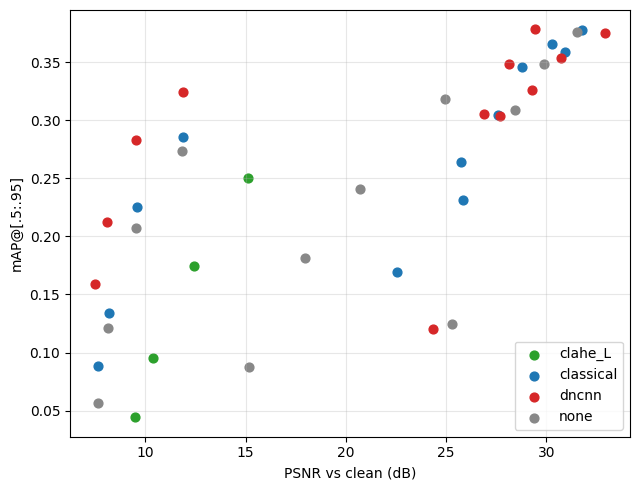
\includegraphics[width=\linewidth]{fig18_psnr_vs_map.png}
\caption{PSNR against mAP (main sweep, 40 runs).}
\label{fig:psnrmap}
\end{subfigure}\hfill
\begin{subfigure}[b]{0.56\linewidth}
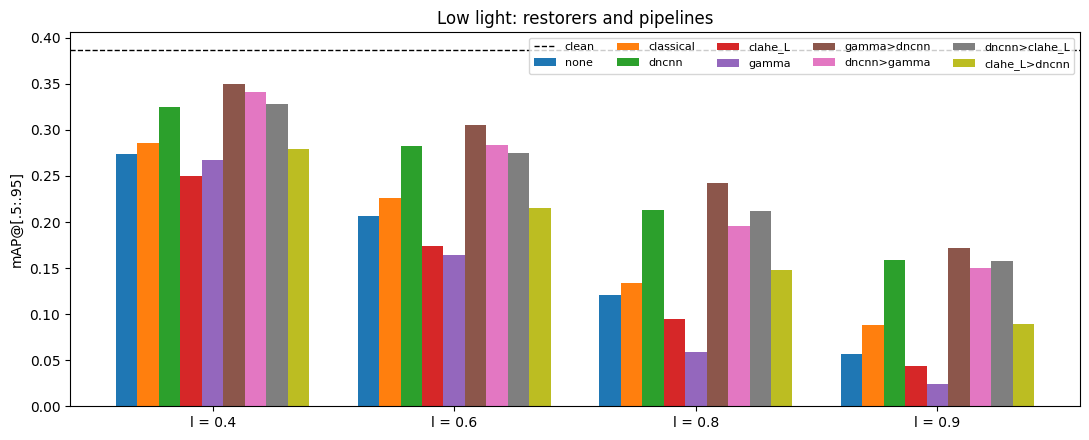
\includegraphics[width=\linewidth]{fig26_low_light_pipelines.png}
\caption{Low light: every restorer and pipeline.}
\label{fig:lowlight}
\end{subfigure}
\caption{(a) PSNR and mAP correlate across conditions because severity lowers both, but within a low-light condition the ordering reverses. (b) Brightening alone (gamma) and CLAHE fall below no restoration; brightening followed by DnCNN is best at every level.}
\label{fig:proxy}
\end{figure}

Across all 64 restored runs, PSNR and mAP correlate (Spearman 0.76), but mostly because severity lowers both (\figref{fig:psnrmap}). What matters when choosing a method is the ranking within one condition. There, PSNR and mAP order restorer pairs the same way on Gaussian noise (1 of 24 pairs reversed, the BM3D--DnCNN near-tie at $\sigma=35$) and JPEG (2 of 12), but reverse 63 of 144 pairs in low light. Among the main-sweep methods, the highest-PSNR method in every low-light condition (CLAHE) is the worst for detection (H5 confirmed). PSNR there is dominated by the brightness gap, while the detector is more sensitive to noise.

The disagreement is starker at the level of individual images. Across all 52 restored runs, the per-image Spearman correlation between a restorer's PSNR gain and its AP gain lies between $-0.14$ and $+0.21$ (median 0.03). Even at $\sigma = 50$, where DnCNN improves AP on 91\% of images, it lowers AP on 5\%, and nothing in the pixels flags which ones.

\subsection{Low light: brighten and denoise, in which order?}
\label{sec:lowlight}
If contrast enhancement fails because it amplifies noise, removing the noise should make brightening useful. \figref{fig:lowlight} confirms this. The blind gamma curve alone raises PSNR by 3.8--6.4\,dB but lowers mAP (0.059 against 0.121 unrestored at $\ell = 0.8$). Brightening followed by DnCNN is the best method at every level, clearly better than DnCNN alone ($+0.013$ to $+0.030$ image-averaged AP), and recovers 35--67\% of the lost mAP. Order matters: brightening first beats denoising first at every level (0.242 against 0.196 mAP at $\ell=0.8$). Brightening first scales the noise up into the range DnCNN was trained on, where it removes it well; denoising first leaves faint residual noise that the gamma curve then amplifies. CLAHE first is the worst order, plausibly because its tile-wise contrast changes make the noise strength vary across the image, unlike the uniform noise DnCNN expects. With these pipelines included, PSNR still prefers the wrong method at $\ell=0.8$ and 0.9.

\subsection{Which object sizes suffer?}
\label{sec:sizes}

\begin{table}[t]
\centering\small
\caption{AP kept after damage (damaged / clean) and share of the loss recovered by the best restorer for that damage, by COCO object size (small $<32^2$ px, large $>96^2$ px).}
\label{tab:sizes}
\begin{tabular}{@{}lccc|ccc@{}}
\toprule
 & \multicolumn{3}{c|}{AP kept} & \multicolumn{3}{c}{Loss recovered} \\
Condition (restorer) & Small & Medium & Large & Small & Medium & Large \\
\midrule
Gaussian $\sigma=25$ (DnCNN) & 58\% & 68\% & 65\% & 87\% & 65\% & 94\% \\
Gaussian $\sigma=50$ (DnCNN) & 25\% & 30\% & 24\% & 75\% & 68\% & 79\% \\
JPEG $q=10$ (bilateral) & 33\% & 39\% & 28\% & 25\% & 35\% & 46\% \\
Low light $\ell=0.8$ (DnCNN) & 22\% & 37\% & 33\% & 35\% & 32\% & 38\% \\
\bottomrule
\end{tabular}
\end{table}

At moderate levels, noise and darkness hurt small objects most (\tabref{tab:sizes}); a small object is only a few pixels across, so the same noise covers a larger share of its detail. Heavy compression hurts large objects most, and the bilateral filter helps them most (46\%) and small objects least (25\%): smoothing block edges restores the outline of an object that spans many blocks, but not detail inside a small object that falls within one or two. Small-object AP is low (0.197 clean), so these differences are indicative.

\subsection{What the denoiser learned}
\label{sec:interp}

\begin{figure}[t]
\centering
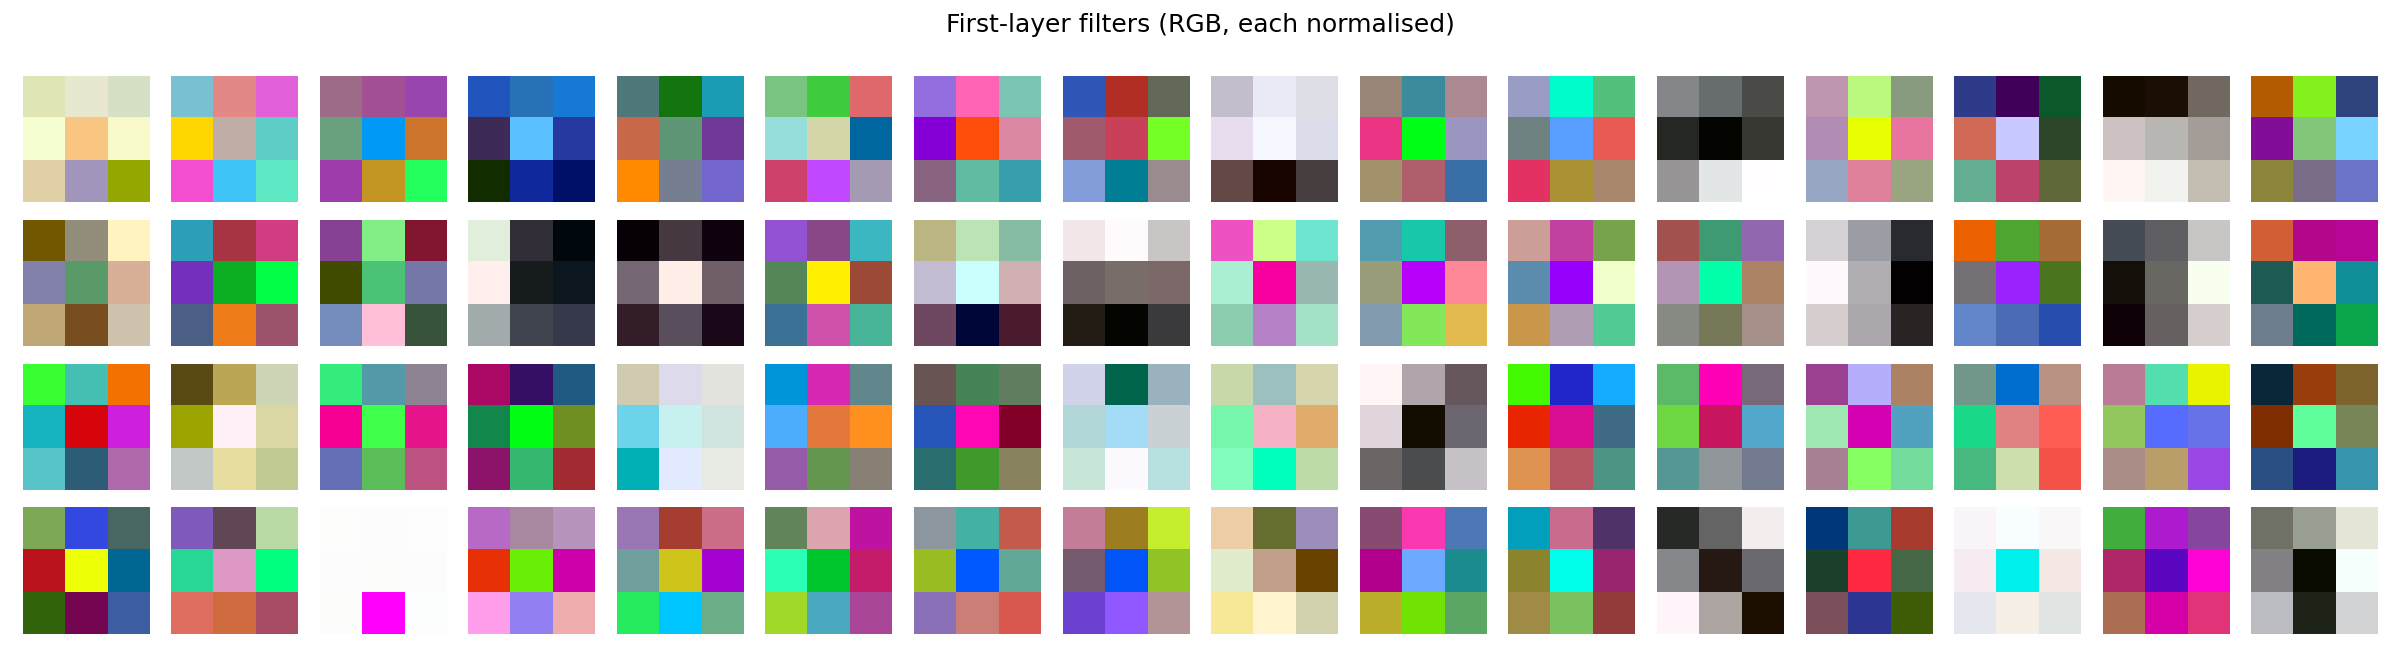
\includegraphics[width=\linewidth]{fig19_filters.png}\\[4pt]
\begin{subfigure}[b]{0.44\linewidth}
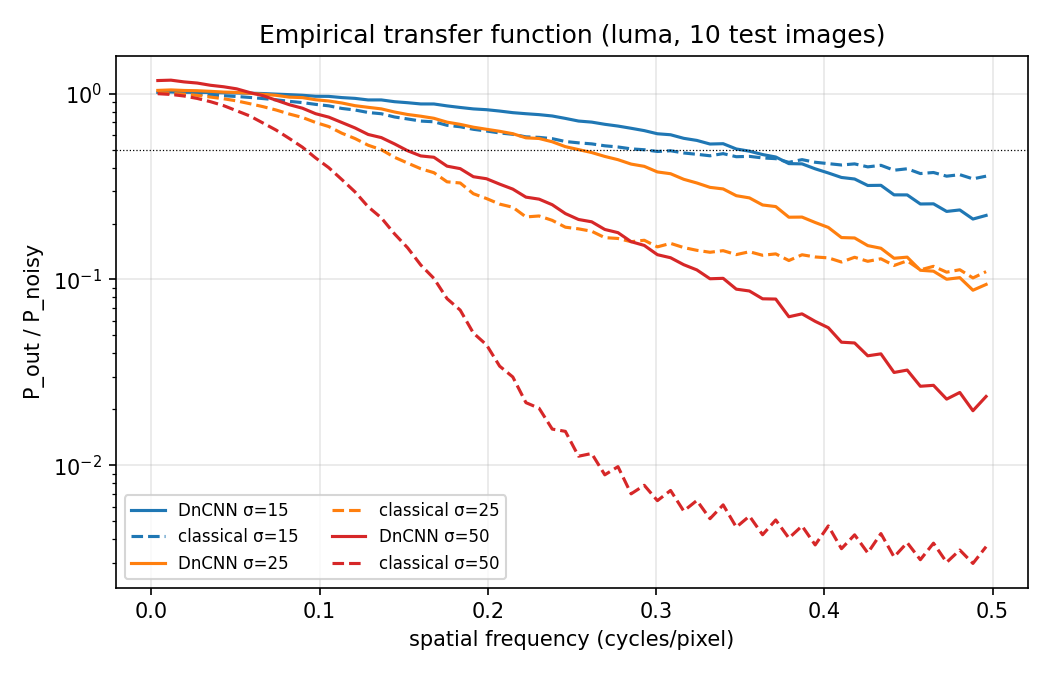
\includegraphics[width=\linewidth]{fig21_transfer_function.png}
\caption{Average transfer function.}
\end{subfigure}\hfill
\begin{subfigure}[b]{0.5\linewidth}
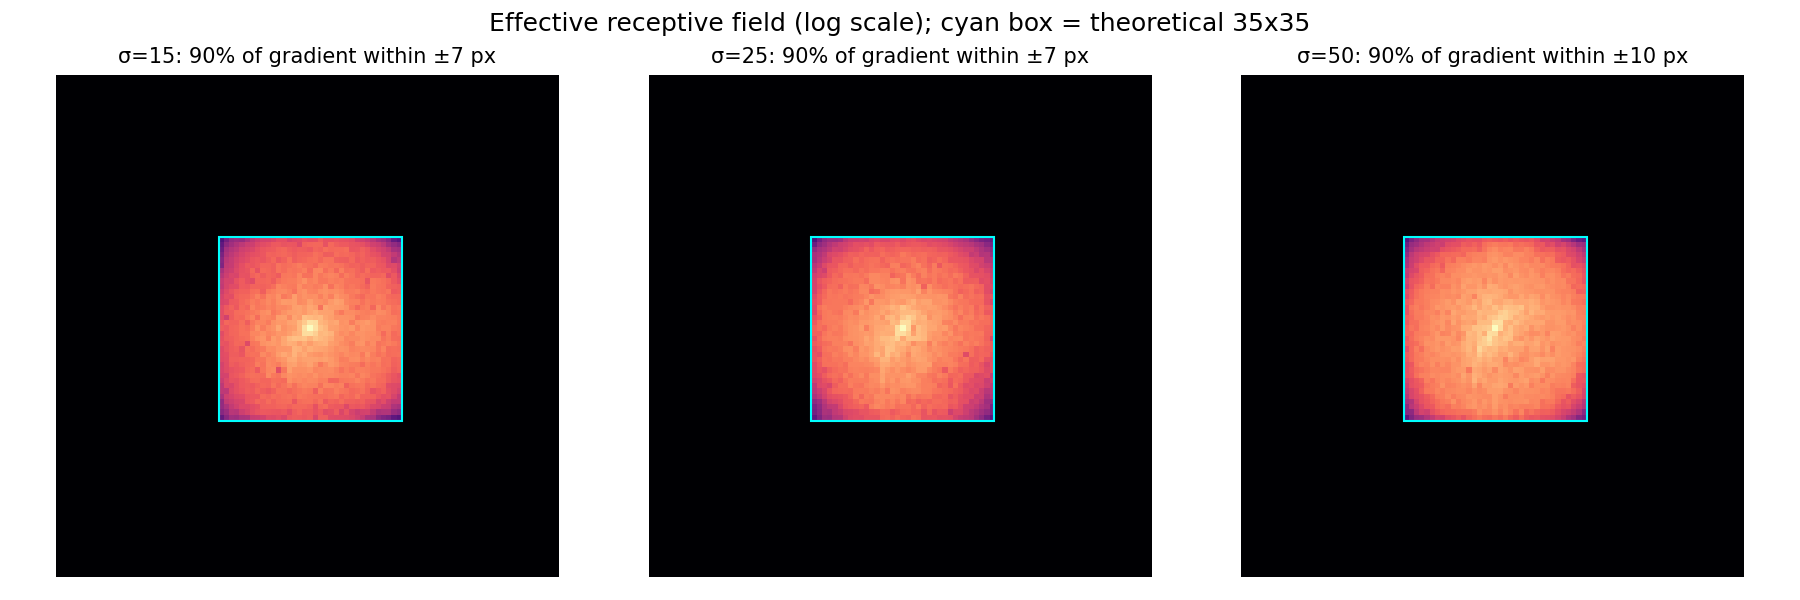
\includegraphics[width=\linewidth]{fig20_receptive_field.png}
\caption{Effective receptive field at $\sigma = 15, 25, 50$.}
\end{subfigure}
\caption{Inside the trained DnCNN. Top: the 64 first-layer filters (RGB, each normalised); most are colour-opponent. (a) DnCNN (solid) keeps more mid and high frequencies than the best classical filter (dashed) at every $\sigma$; the dotted line marks half power. (b) The region that influences an output pixel widens as noise grows.}
\label{fig:interp}
\end{figure}

\paragraph{Filters.} Only 9 of the 64 first-layer filters are close (cosine $\geq 0.8$) to a textbook kernel: 6 Sobel, 1 Laplacian, 1 Gaussian and 1 identity. The typical filter puts 79\% of its energy on differences between colour channels, and 43 of 64 are mostly colour-opponent (\figref{fig:interp}). The network was never told about colour spaces, yet it learned the separation our colour-space experiment found by hand (Appendix~\ref{app:classical}): image detail lives in brightness, so colour differences can be treated more aggressively.

\paragraph{Receptive field and frequency response.} Although each output pixel can see a $35\times35$ window, 90\% of the gradient mass lies within $\pm7$ pixels at $\sigma = 15$ and 25, widening to $\pm10$ at $\sigma=50$: the network infers the noise level and enlarges its neighbourhood accordingly. The frequency at which output power falls to half is 0.355, 0.254 and 0.152 cycles/pixel at $\sigma = 15, 25, 50$, against 0.293, 0.137 and 0.098 for the best classical filter. DnCNN's cutoff is up to $1.9\times$ higher, and at $\sigma = 50$ it passes about six times more of the highest frequencies, which carry edges and texture. This is the most likely reason a strong denoiser recovers so much mAP on noise.

\begin{table}[t]
\centering\small
\caption{DnCNN's predicted residual on 20 test images. Edge leak is the correlation between residual size and clean-image edge strength; near zero means the network does not remove structure.}
\label{tab:residual}
\begin{tabular}{@{}lcccc@{}}
\toprule
Input & PSNR in (dB) & PSNR out (dB) & Change (dB) & Edge leak \\
\midrule
Gaussian $\sigma=25$ & 20.55 & 31.11 & $+10.56$ & $-0.02$ \\
Salt and pepper 0.05 & 17.92 & 18.15 & $+0.24$ & $-0.01$ \\
JPEG $q=10$ & 25.65 & 24.56 & $-1.08$ & 0.05 \\
Blur $\sigma=2$ & 24.31 & 22.58 & $-1.73$ & 0.05 \\
Low light 0.8 & 8.68 & 8.58 & $-0.10$ & 0.05 \\
\bottomrule
\end{tabular}
\end{table}

\paragraph{Residuals out of distribution.} On Gaussian noise the predicted residual correlates 0.935 with the true noise and contains no edges (\tabref{tab:residual}). On salt-and-pepper noise the network does almost nothing. On JPEG and blur the residual is near zero almost everywhere but has a few large, saturated spikes along strong edges, which appear in the output as streaks (\figref{fig:residual}); these failures explain why DnCNN never helps on JPEG. In low light the residual looks like noise and the output is cleaner but just as dark: DnCNN removes the noise and leaves the brightness, so PSNR does not move while mAP rises.

\begin{figure}[t]
\centering
\begin{subfigure}[b]{0.36\linewidth}
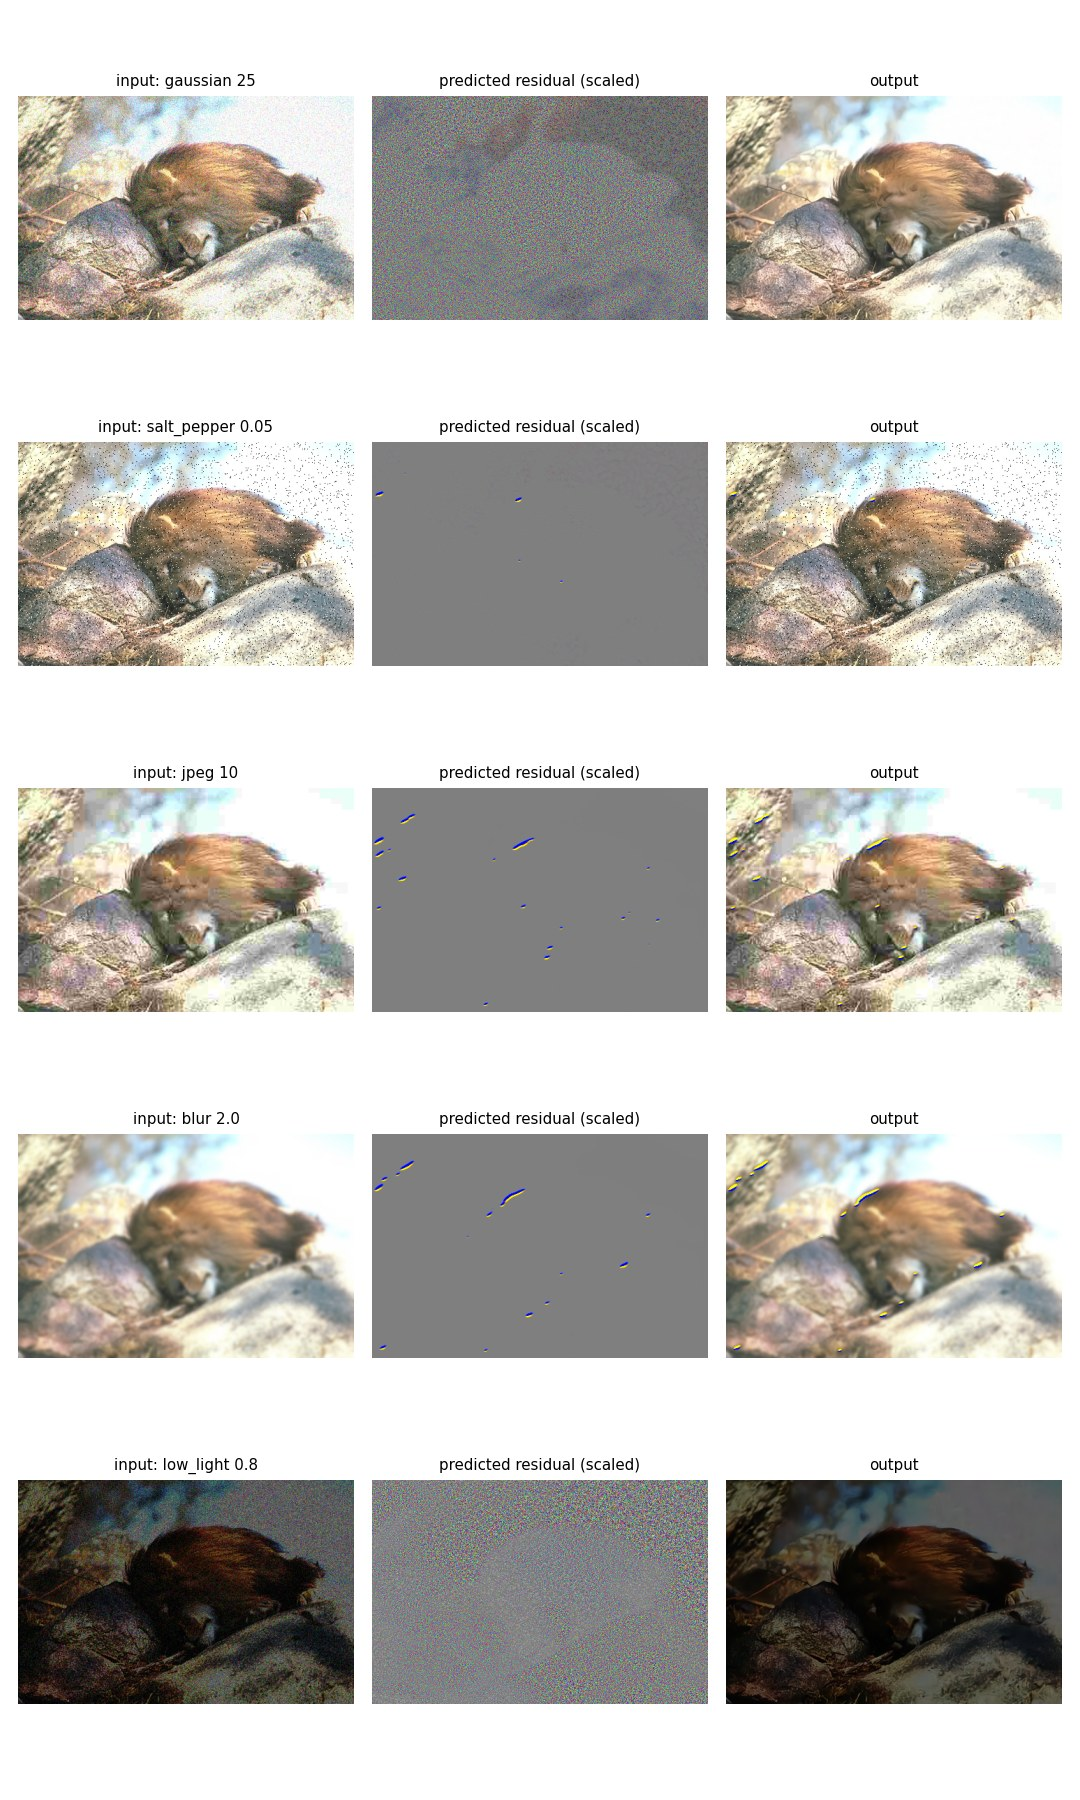
\includegraphics[width=\linewidth]{fig22_residual_probes.jpg}
\caption{Input, residual, output.}
\label{fig:residual}
\end{subfigure}\hfill
\begin{subfigure}[b]{0.6\linewidth}
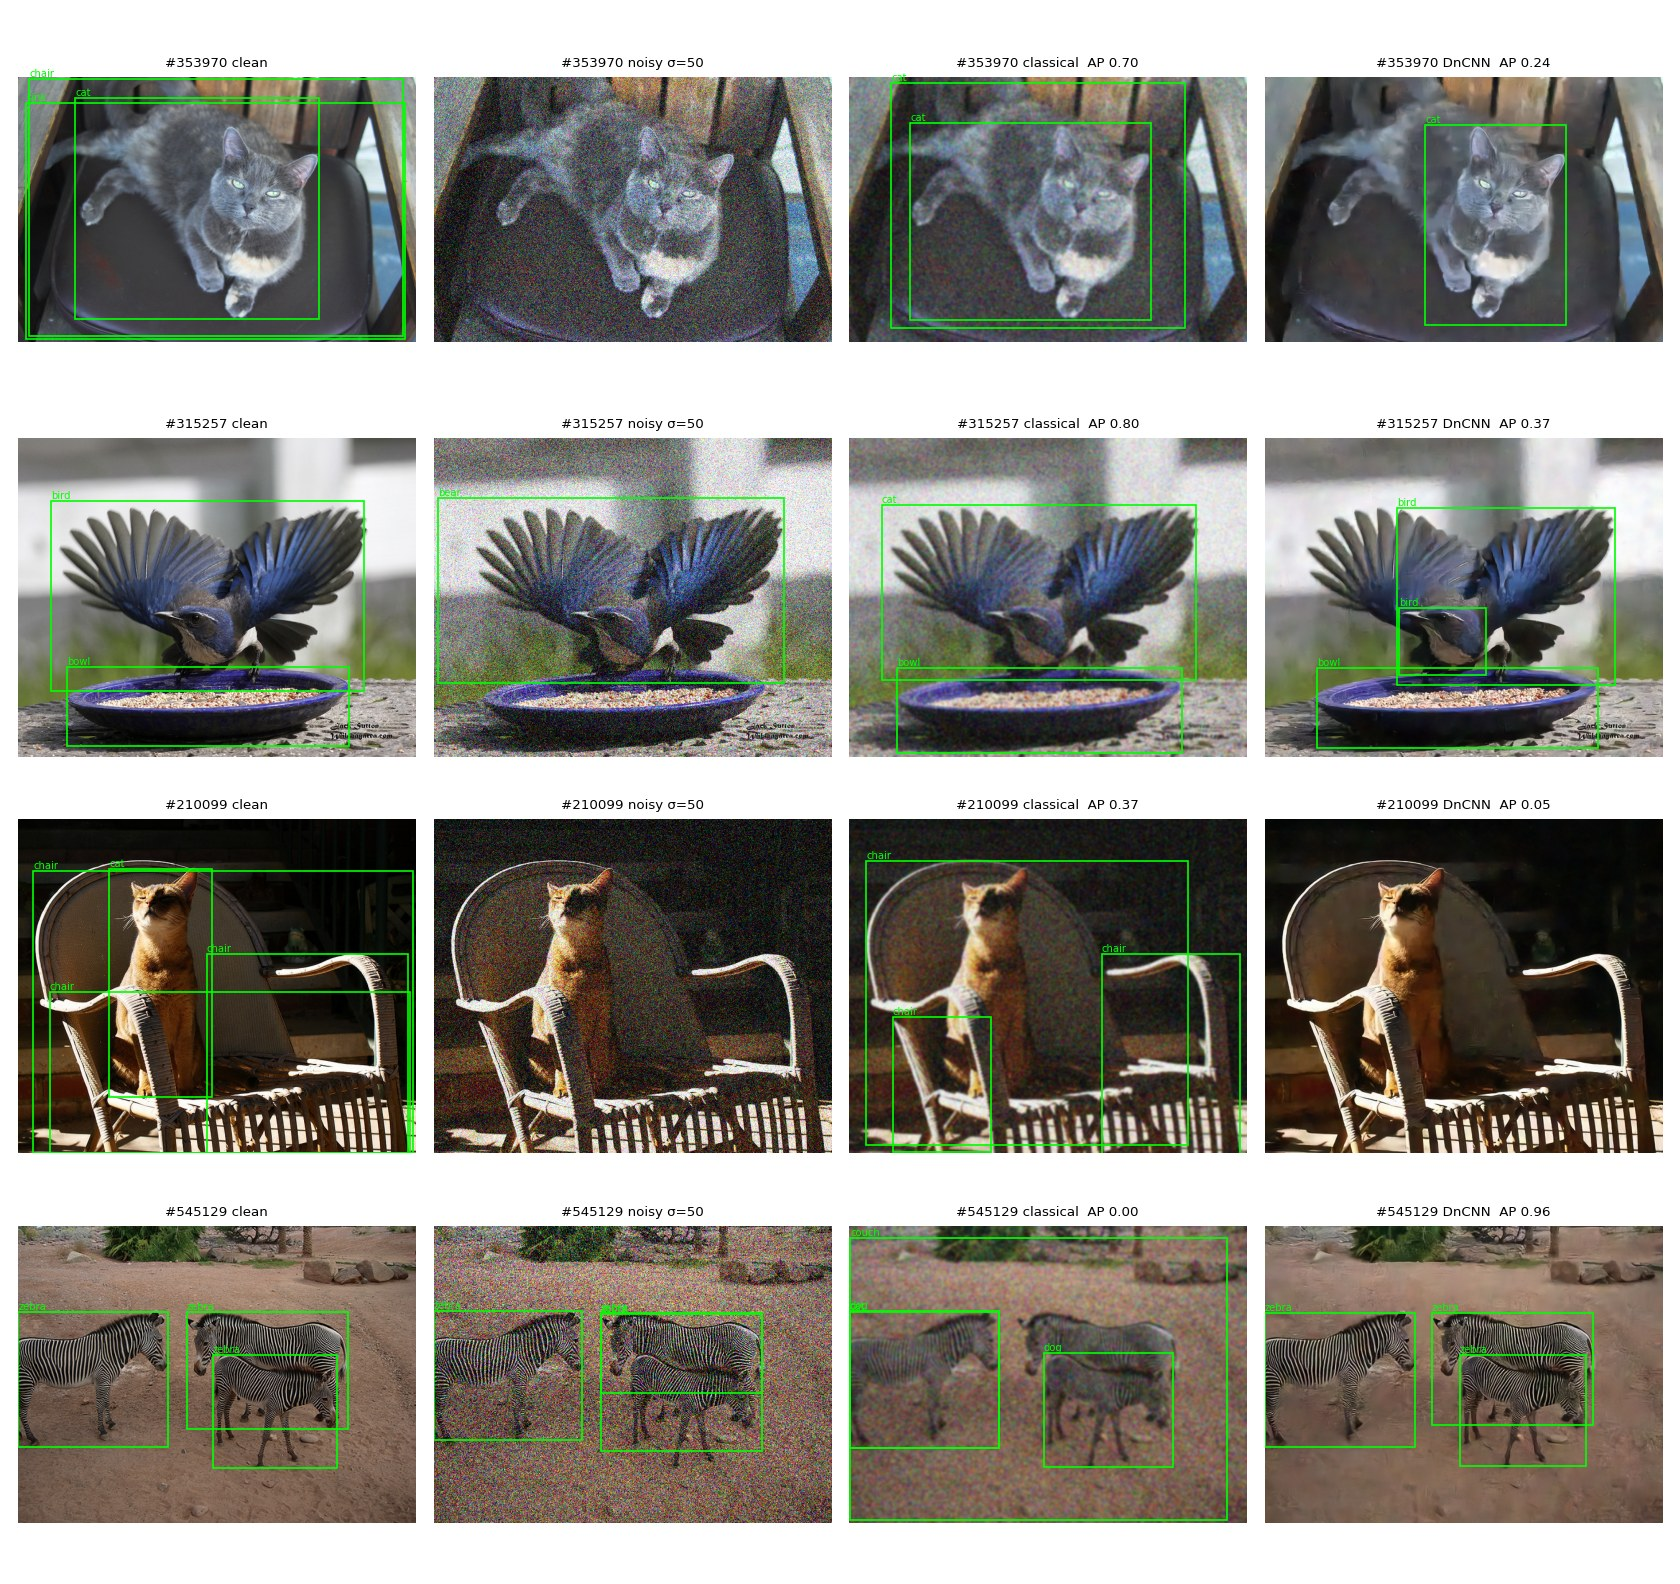
\includegraphics[width=\linewidth]{fig23_failure_gallery.jpg}
\caption{$\sigma=50$: clean, noisy, classical, DnCNN with detections.}
\label{fig:gallery}
\end{subfigure}
\caption{(a) DnCNN's residual for five kinds of damage: noise-like on Gaussian noise and low light, a few saturated streaks along edges on JPEG and blur. (b) Images where DnCNN has the higher PSNR but the lower AP: it over-smooths low-contrast texture the detector needs (first three rows); the last row shows the opposite case.}
\label{fig:failures}
\end{figure}

\paragraph{Where higher PSNR still loses.} At $\sigma=50$ DnCNN has higher PSNR than the tuned filter on every image but lower AP on 40 of 300 (13\%). In these cases its output is clean but over-smoothed in flat, low-contrast regions such as fur and background, and the detector misses objects or draws smaller boxes (\figref{fig:gallery}).

\subsection{Hypotheses}

\begin{table}[H]
\centering\small
\caption{Outcome of the hypotheses stated before the detection experiments.}
\label{tab:hyp}
\begin{tabular}{@{}p{0.36\linewidth}p{0.17\linewidth}p{0.4\linewidth}@{}}
\toprule
Hypothesis & Outcome & Evidence \\
\midrule
H1: mAP falls steadily with severity & Confirmed & falls at every step, to 0.088 / 0.125 / 0.056 \\
H2: both restorers help on noise, DnCNN more & Confirmed, qualified & DnCNN 70--83\% vs tuned 27--60\%; tie with BM3D \\
H3: little recovered on JPEG; DnCNN may hurt & Confirmed except $q \leq 30$ & DnCNN never helps; bilateral 41--48\% at $q=30$, 10 \\
H4: CLAHE helps most in low light & Rejected & CLAHE $-4\%$ to $-21\%$; gamma$\to$DnCNN best \\
H5: best-PSNR restorer is not always best-mAP & Confirmed & 63 of 144 low-light pairs reversed \\
\bottomrule
\end{tabular}
\end{table}

% ================================================================= 5 discussion
\section{Discussion}
\label{sec:discussion}

\paragraph{Restoration helps when it removes what the detector is sensitive to.} The detector is most sensitive to random noise, and a strong denoiser removes it while keeping the mid and high frequencies that carry edges and texture. Restorations that remove nothing the detector cares about (DnCNN on JPEG) or that amplify what it cares about most (brightening, CLAHE) do not help, regardless of their pixel scores.

\paragraph{Darkness is not the problem; amplified noise is.} The residual analysis (\secref{sec:interp}) and the low-light pipelines (\secref{sec:lowlight}) agree: brightness can be restored usefully once the noise is dealt with, and brightening \emph{before} denoising works best because it presents the denoiser with noise of the strength it was trained on. This is a cheap, training-free improvement for a denoiser trained only on Gaussian noise.

\paragraph{PSNR is a usable guide between methods, not between images.} Within noise and compression, PSNR orders methods almost as mAP does, so it is a reasonable proxy for choosing a method on average. It fails when restoration changes brightness or contrast, and at the level of individual images it carries almost no information about detection. This suggests measuring restoration in the detector's own feature space, which we leave to future work.

\paragraph{Learned versus classical.} On PSNR, DnCNN's advantage over BM3D is clear and grows with noise. For detection the two are indistinguishable. A study that compares a learned restorer only with simple filters would overstate the benefit of learning; including the strongest classical baseline changes the conclusion.

% ================================================================= 6 limitations
\section{Limitations}
\label{sec:limits}
\begin{itemize}
  \item One detector (YOLOv8n) and 300 COCO images. The bootstrap uses image-averaged AP rather than COCO mAP itself, and some small differences remain unresolved, such as DnCNN against BM3D and the bilateral filter at JPEG $q = 50$--70.
  \item All degradations are synthetic. Real sensor noise is signal-dependent and spatially correlated, and real low-light images are not a simple tone curve plus noise.
  \item DnCNN was trained only on Gaussian noise, so its JPEG, blur and low-light results measure generalisation, not what a learned restorer trained for those damages could do.
  \item The tuned filters and BM3D were given the true severity, which favours them; DnCNN's margins over them are therefore conservative.
  \item The interpretability measures are averages over 10--20 images, and only first-layer filters were inspected directly.
\end{itemize}

% ================================================================= 7 conclusion
\section{Conclusion and Future Work}
\label{sec:conclusion}
Restoration does help a pretrained detector, but only when it removes the kind of damage the detector is sensitive to. A strong denoiser recovers about three-quarters of the mAP lost to Gaussian noise, whether it is learned (DnCNN) or classical (BM3D). Compression artifacts are worth repairing only at strong compression. In low light, pixel metrics rank methods in the wrong order, and brightening followed by denoising is best. PSNR is a reasonable guide to choosing a method on average when damage is additive noise or compression, but not when restoration changes brightness, and almost never for an individual image. Restoration meant for machines should therefore be evaluated, and ideally optimised, with the downstream task metric.

Future work: training the restorer on JPEG and low-light damage; comparing restoration with fine-tuning the detector on damaged images; a second detector and real photographs such as ExDark~\citep{loh2019exdark}; and task-driven restoration that measures where damage enters the detector's features and trains a denoiser to undo it~\citep{liu2018denoising,diamond2021dirty}.

\section*{Code and Data Availability}
All notebooks, saved outputs, the trained DnCNN checkpoint and the analysis scripts are available at \url{https://github.com/onigiri4711/degrade-restore-detect}. All randomness is seeded, and the COCO subset ids are saved with the detection results.

\section*{Use of AI Assistance}
An AI assistant (Claude, Anthropic) was used for planning the study, scaffolding notebooks, debugging, writing analysis scripts and drafting this manuscript. All experiments were run by the author on Kaggle, and every reported number was checked against the saved notebook outputs.

\bibliographystyle{plainnat}
\bibliography{refs}

% ================================================================= appendix
\clearpage
\appendix

\section{Components Built from Scratch}
\label{app:scratch}

\paragraph{JPEG codec.} We implement the lossy core of baseline JPEG~\citep{wallace1992jpeg} in NumPy: RGB to YCbCr, 4:2:0 chroma subsampling, $8\times8$ blocks, the 2-D DCT as $F = C B C^\top$ with an orthonormal $C$, quantisation with the standard tables scaled by quality, zigzag ordering, and an entropy estimate of JPEG's own symbols (DC differences and run-length (run, size) pairs). At equal quality our PSNR is within 0.05\,dB of libjpeg up to $q=90$ (\figref{fig:jpeg}); our size estimate is $0.86\times$ the real file size, an idealised lower bound without Huffman tables and headers. The first 15 of 64 DCT coefficients hold 95.7\% of luma energy, and 73.8\% of coefficients quantise to zero at $q = 50$. At $q=10$, pixel steps across block boundaries are $2.1\times$ those inside blocks. Bilinear chroma upsampling matters: nearest-neighbour upsampling cost 4.9\,dB at $q = 95$.

\begin{figure}[h]
\centering
\begin{subfigure}[b]{0.3\linewidth}
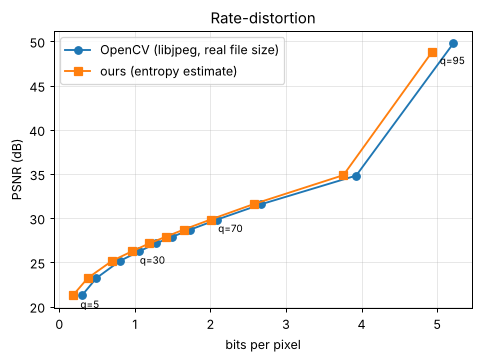
\includegraphics[width=\linewidth]{fig12_rate_distortion.png}
\caption{Rate--distortion.}
\end{subfigure}\hfill
\begin{subfigure}[b]{0.66\linewidth}
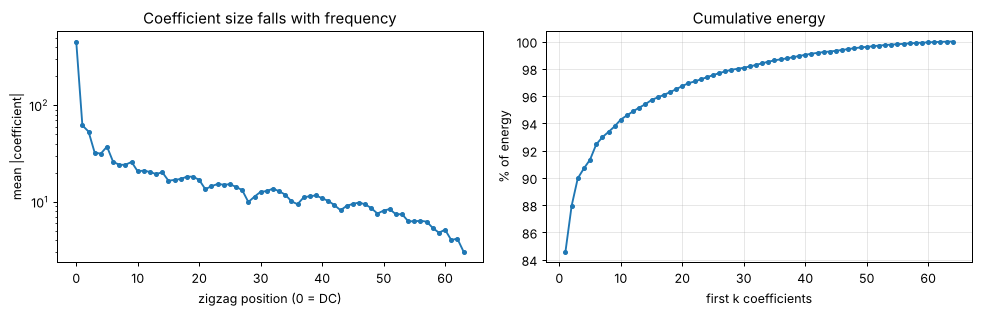
\includegraphics[width=\linewidth]{fig11_dct_energy.png}
\caption{Coefficient size and cumulative energy.}
\end{subfigure}\\[4pt]
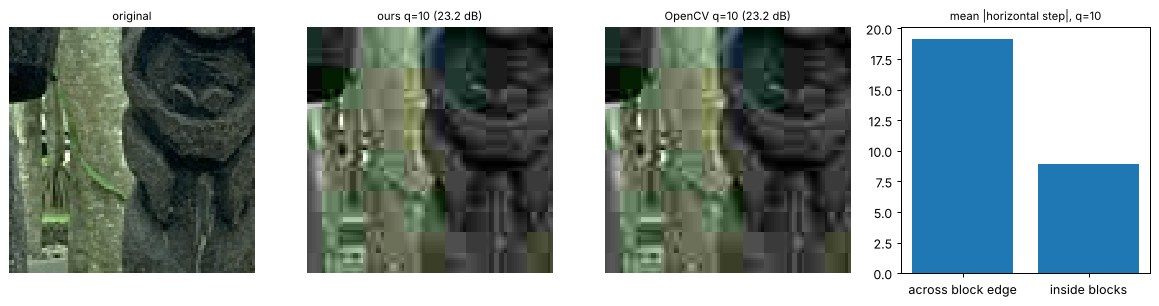
\includegraphics[width=0.7\linewidth]{fig13_jpeg_artifacts.jpg}
\caption{Our JPEG codec. (a) PSNR against bits per pixel, ours (estimated size) and OpenCV's libjpeg (real size). (b) Energy compaction in the DCT. Bottom: original, ours and OpenCV at $q = 10$, with the blocking measure.}
\label{fig:jpeg}
\end{figure}

\paragraph{Convolution layer.} We derive and implement the forward pass and the gradients with respect to input, weights and bias, once with explicit loops and once with im2col. The forward pass matches SciPy's cross-correlation to $10^{-10}$; analytic gradients match central-difference gradients with relative error at most $7\times10^{-10}$ at strides 1 and 2, while a deliberately wrong kernel orientation gives 0.71. im2col is $248\times$ faster than element-wise loops. A three-layer denoiser built only from this layer, trained for 400 Adam steps on $32\times32$ grayscale patches at $\sigma=25$, raises a held-out crop from 20.65 to 25.43\,dB (\figref{fig:numpy}).

\begin{figure}[h]
\centering
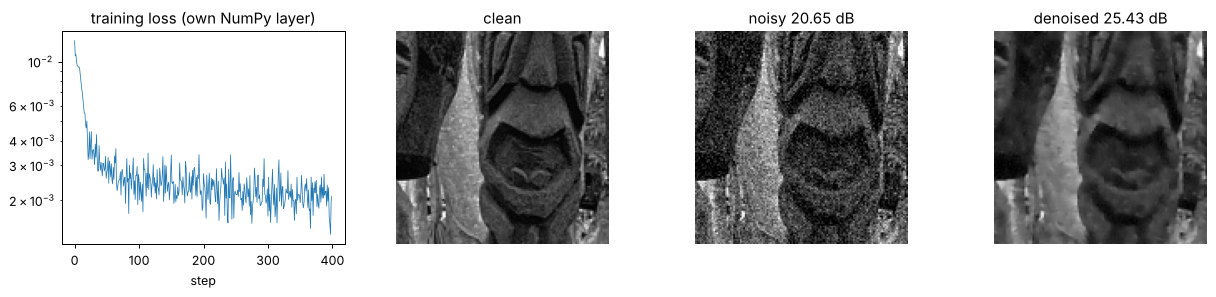
\includegraphics[width=0.8\linewidth]{fig14_numpy_denoiser.png}
\caption{A three-layer denoiser built from the NumPy convolution layer: training loss and a $\sigma = 25$ example.}
\label{fig:numpy}
\end{figure}

\section{Classical Experiments}
\label{app:classical}

\begin{table}[h]
\centering\small
\caption{Best tuned classical filter at the middle severity of each degradation (96 BSD500 test images).}
\label{tab:classical}
\begin{tabular}{@{}llcccc@{}}
\toprule
Degradation & Severity & Noisy (dB) & Best filter & Best (dB) & Gain (dB) \\
\midrule
Salt and pepper & $a = 0.05$ & 18.00 & median & 28.64 & $+10.64$ \\
Poisson & $p = 20$ & 17.56 & bilateral & 25.15 & $+7.59$ \\
Gaussian & $\sigma = 25$ & 20.53 & bilateral & 27.56 & $+7.03$ \\
JPEG & $q = 50$ & 31.01 & bilateral & 31.36 & $+0.35$ \\
Colour cast & $s = 0.3$ & 20.03 & NL-means & 20.15 & $+0.13$ \\
Low light & $\ell = 0.6$ & 9.86 & Gaussian & 9.89 & $+0.03$ \\
Blur & $\sigma = 1.5$ & 25.76 & none & 25.76 & 0 \\
\bottomrule
\end{tabular}
\end{table}

\begin{figure}[h]
\centering
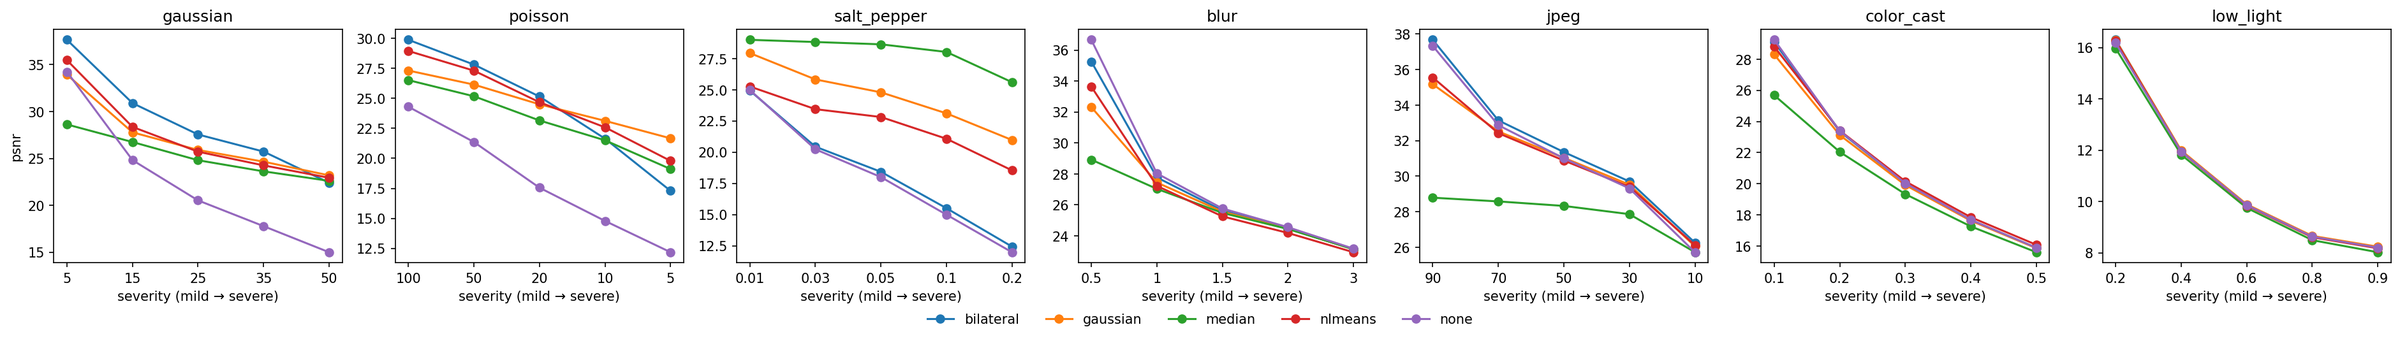
\includegraphics[width=\linewidth]{fig02_severity_psnr.png}
\caption{PSNR against severity for every degradation and classical filter.}
\label{fig:severity}
\end{figure}

\paragraph{Classical filters.} \tabref{tab:classical} and \figref{fig:severity} show the split between noise, which filters repair, and the other degradations, which they cannot. At the heaviest noise, plain Gaussian blur beats edge-preserving filters, because noise as large as the edges is preserved too. Blind NL-means, which estimates $\sigma$ from the image~\citep{donoho1994wavelet}, loses only 0.04--0.31\,dB against its oracle version from $\sigma = 15$ to 50.

\paragraph{Colour space.} Noise is spread almost evenly across YCrCb channels (measured $0.667\sigma$, $0.658\sigma$ and $0.625\sigma$, matching $\sigma\lVert w\rVert_2$), but image detail is concentrated in luma (detail-to-noise ratio 1.27 in Y against 0.06--0.10 in chroma at $\sigma=25$). Smoothing luma gently and chroma strongly with the same Gaussian filter beats equal RGB smoothing on 100\% of images at $\sigma = 15$ and 25 ($+2.07$ and $+1.51$\,dB); the reverse configuration loses 2.4--3.2\,dB (\figref{fig:colour}).

\begin{figure}[h]
\centering
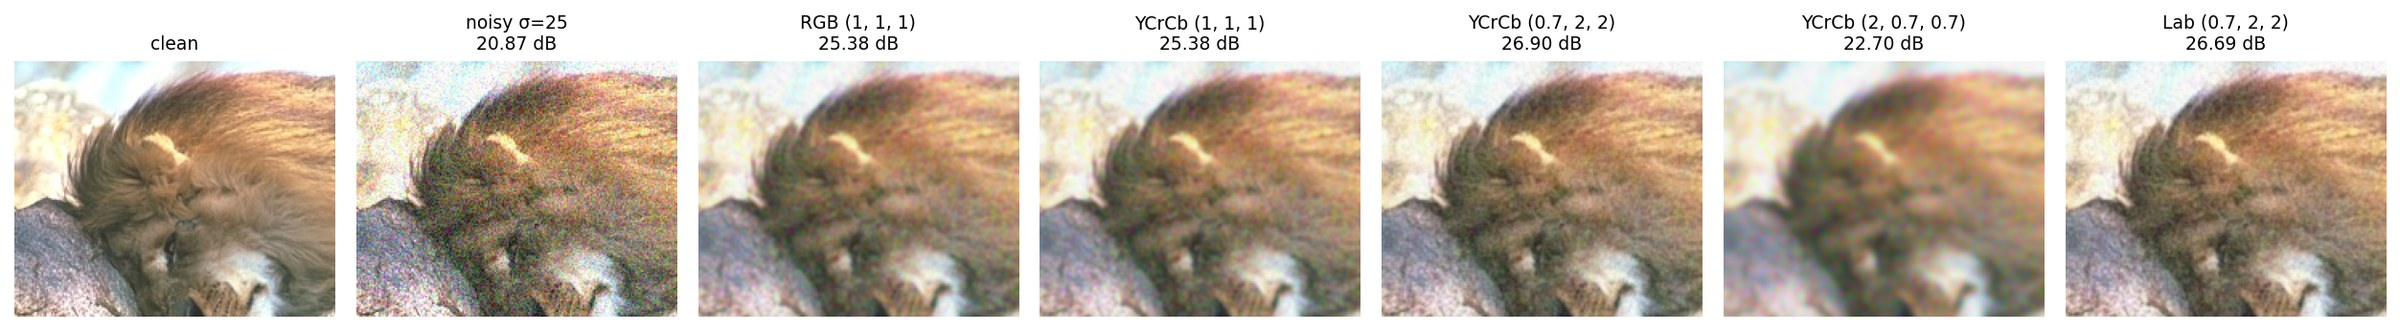
\includegraphics[width=\linewidth]{fig05_colorspace_crop.jpg}
\caption{The same Gaussian blur applied in RGB, YCrCb and Lab at $\sigma = 25$, with per-channel strengths and PSNR.}
\label{fig:colour}
\end{figure}

\paragraph{Contrast enhancement.} At $\ell = 0.6$, histogram equalisation on separate RGB channels multiplies the colour shift by 2.6, while working on Lab's L channel leaves colour unchanged. HE on L wins on PSNR (14.48\,dB) and CLAHE on L on SSIM (0.383), but PSNR stays at 12.8--14.5\,dB because equalisation produces a pleasing tone curve rather than the original values (\figref{fig:contrast}).

\begin{figure}[h]
\centering
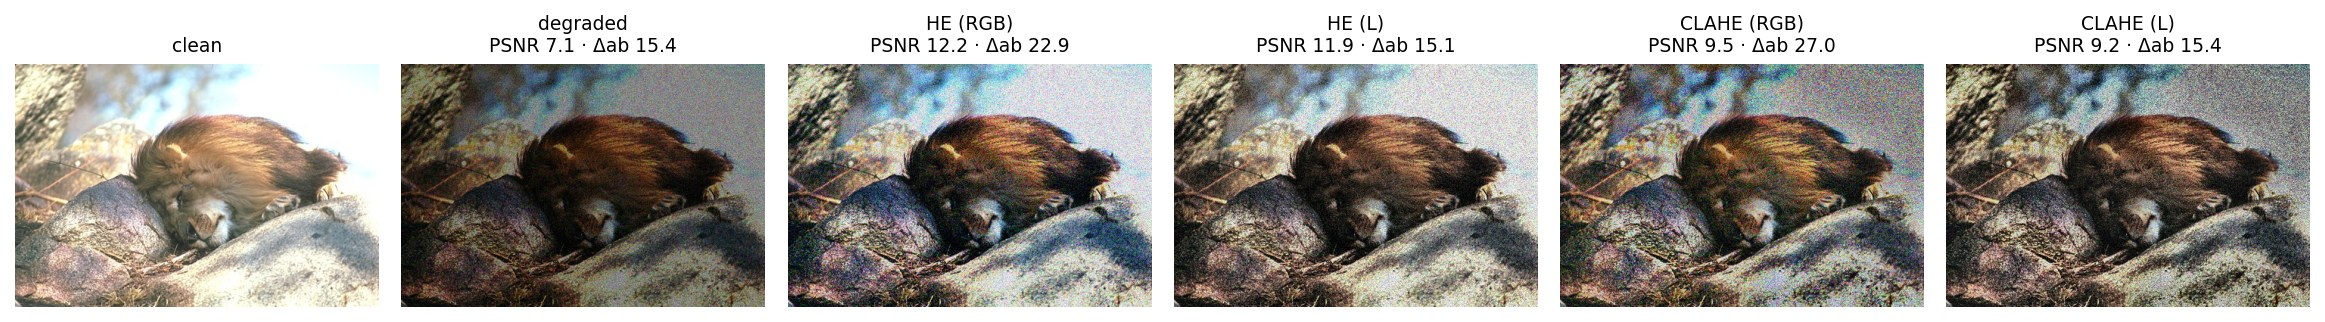
\includegraphics[width=\linewidth]{fig07_contrast_level06.jpg}
\caption{Low light $\ell = 0.6$: degraded input, then HE and CLAHE on RGB and on the L channel.}
\label{fig:contrast}
\end{figure}

\paragraph{Matched inverses.} Gray-world white balance recovers 7.7\,dB at cast strength 0.5, where the best denoiser gains 0.19\,dB. Wiener deconvolution gains up to 9.5\,dB on noise-free blur, where every denoiser makes the image worse; adding noise of $\sigma = 2/255$ moves the best regulariser $K$ from $10^{-4}$ to $10^{-2}$ and cuts the gain to 1.5--1.8\,dB (\figref{fig:wiener}).

\begin{figure}[h]
\centering
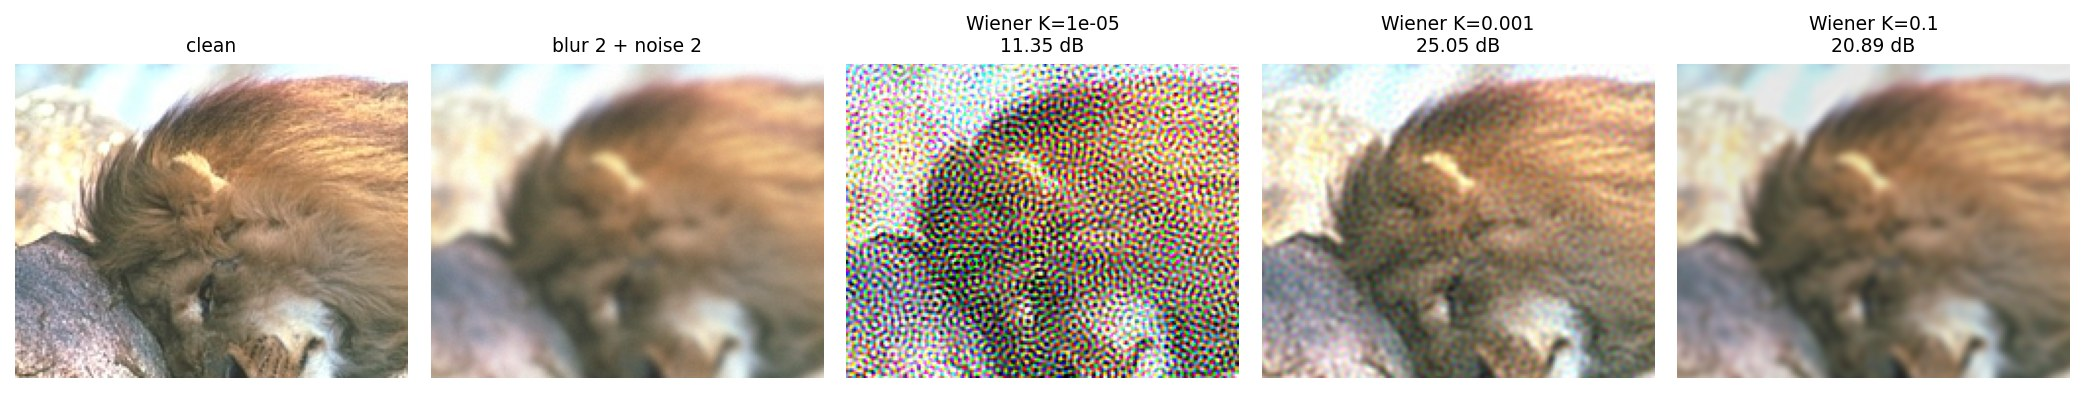
\includegraphics[width=\linewidth]{fig09_wiener.jpg}
\caption{Wiener deconvolution of blur $\sigma = 2$ plus noise for three values of $K$: too small amplifies noise, too large leaves blur.}
\label{fig:wiener}
\end{figure}

\section{DnCNN Training and Examples}
\label{app:dncnn}

\begin{figure}[h]
\centering
\begin{subfigure}[b]{0.62\linewidth}
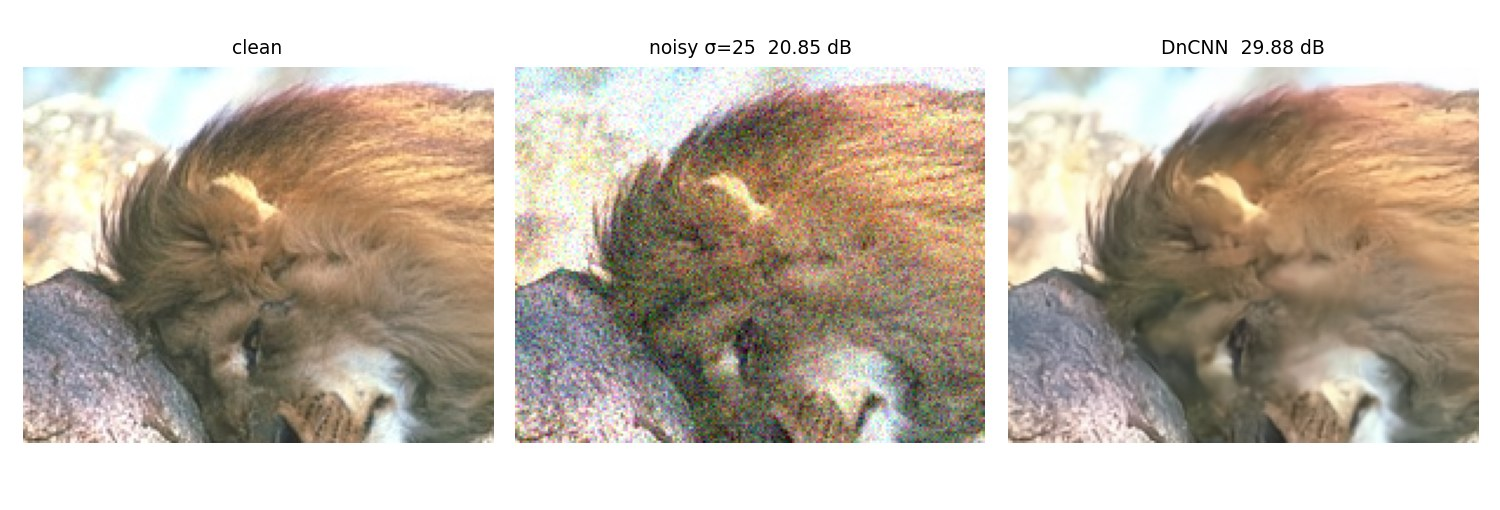
\includegraphics[width=\linewidth]{fig15_dncnn_crop.jpg}
\caption{Clean, noisy (20.85\,dB), DnCNN (29.86\,dB).}
\end{subfigure}\hfill
\begin{subfigure}[b]{0.34\linewidth}
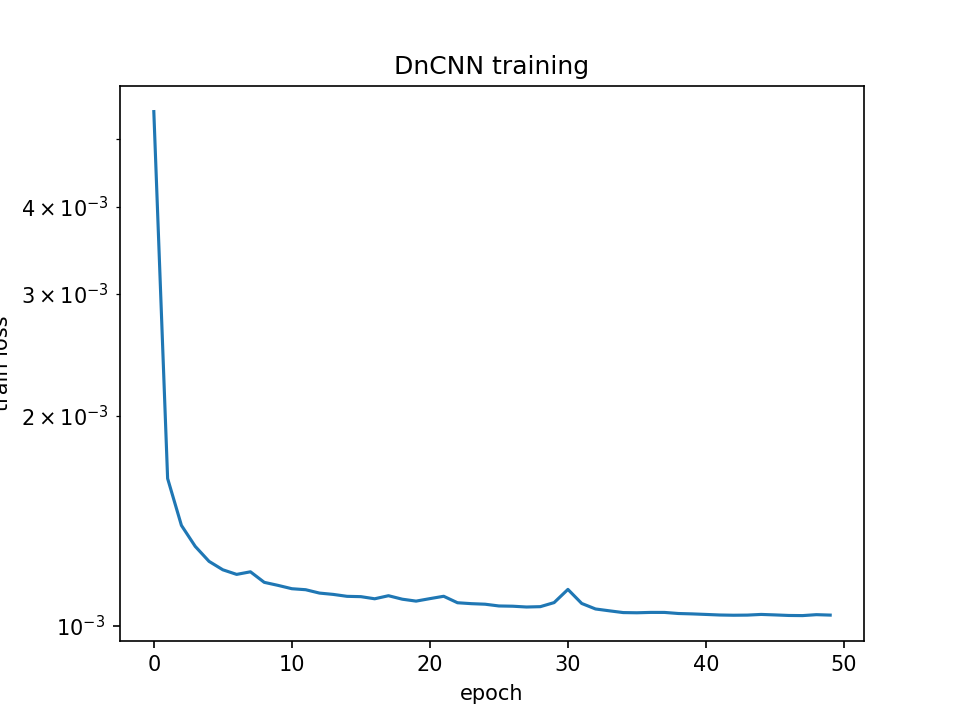
\includegraphics[width=\linewidth]{fig16_dncnn_loss.png}
\caption{Training loss.}
\end{subfigure}
\caption{DnCNN at $\sigma = 25$ and its training curve over 50 epochs. The loss falls below the predict-zero baseline within the first epoch and levels off at $1.04\times10^{-3}$.}
\label{fig:dncnn}
\end{figure}

\end{document}
